\section{Response to Reviewer \#1}

Dear Reviewer 1,\\

Thank you very much for your detailed and constructive comments on our manuscript. We appreciate the reviewer's careful assessment and the positive recognition of the algebraic recovery guarantee in Theorem~2, the combined coding--OTFS--finite-blocklength framework, and the breadth of the simulation study. Your insightful suggestions have been instrumental in improving the quality and clarity of our work. We provide our detailed responses below.

\noindent\rule{17cm}{2.0pt}

%%%%%%%%%%%%%%%%%%%%%%%%%%%%%%%%%%%%%%%%%%%%%%%%%%%%%%%%%%%%%%%%%%%%%%
\subsection{Reviewer Comment-1}
\begin{mdframed}
\begin{quote}
This paper studies a retransmission-free reliability architecture for OTFS-based LEO NTN downlinks. The main idea is to insert a diversity transform between the FEC encoder and the modulator, construct the transform from an MDS/Reed–Solomon code, predict subchannel reliability using ephemeris-driven large-scale channel information, and then exploit the resulting block-erasure structure at the receiver. The paper also develops a finite-blocklength BLER analysis for the OTFS transparent-relay setting and provides simulation results over a range of parameters. Overall, I find the topic timely and the paper technically interesting. The algebraic recovery guarantee in Theorem 2 is the clearest strength of the work, and the combination of coding, OTFS, and finite-blocklength analysis is a meaningful contribution.
The numerical section is also reasonably broad. The manuscript reports good agreement between the analytical BLER approximation and Monte Carlo simulation, shows improvements over non-diversity polar-coded baselines, studies elevation angle, blockage probability, number of subchannels, and Doppler sensitivity, and argues for a latency advantage over HARQ-CC. These are all positive aspects and they make the paper more than a purely mathematical exercise.
That said, I believe the manuscript still needs a substantial revision before it is ready for publication in a transactions journal.
First, the paper's practical validation is not yet strong enough relative to the strength of its claims. A central component of the framework is the ephemeris-driven prediction layer, but the current analysis assumes effectively perfect ephemeris knowledge and does not provide a sensitivity study with respect to prediction error, user-location error, atmospheric-model mismatch, or prediction horizon. Since the diversity transform is proactively selected based on predicted outage patterns, the robustness of the design to prediction mismatch is essential. Please add a dedicated robustness study showing how BLER/latency degrade when the predicted reliability scores are imperfect.


\end{quote}

\end{mdframed}


\subsection{Response}

We thank the reviewer for this important suggestion. A dedicated robustness analysis has been added to the revised manuscript, comprising three elements: (i) a new analytical subsection, Section~IV-E, ``Sensitivity to Prediction Imperfections,'' that models the combined prediction error from ephemeris errors, UE location uncertainty, and atmospheric model mismatch as a log-normal perturbation on the predicted SNR; (ii) a new Proposition (Proposition~\ref{prop:bler_imperfect}) providing a closed-form expression for the per-subchannel BLER under imperfect prediction; and (iii) two new simulation figures---Fig.~\ref{fig:bler_robustness} and Fig.~\ref{fig:latency_robustness}---showing that the system BLER degrades gracefully (from $0.105$ to $0.139$ at $\sigma_p = 4$~dB) and the latency advantage over HARQ-CC is preserved with less than a twofold penalty, even under severe prediction mismatch. The prediction horizon contributes negligible additional mismatch since LEO orbital geometry changes over tens of seconds while the system latency is on the order of milliseconds. In Section~IV, we now write:

\begin{quote}
{\color{blue}
\subsection{Sensitivity to Prediction Imperfections}

The prediction framework in Section~\ref{sec:ephemeris_prediction}
assumes perfect ephemeris knowledge and accurate UE positioning.
In practice, three sources of uncertainty introduce discrepancies
between the predicted and actual subchannel SNRs:
(i)~orbital ephemeris errors, which produce elevation-angle
offsets propagating through the slant-range
and atmospheric-loss models in~\eqref{eq:predicted_path_loss};
(ii)~UE location uncertainty, which introduces additional
elevation-angle error; and
(iii)~atmospheric model mismatch, arising from real-time
variability in tropospheric and ionospheric conditions that
deviates from the statistical models used
in~\eqref{eq:predicted_path_loss}.  The combined prediction error for subchannel~$i$ is represented as $\delta_i \sim \mathcal{N}(0, \sigma_p^2)$, where $\sigma_p$~(dB) characterises the aggregate uncertainty. Incorporating this prediction error, the predicted end-to-end SNR for subchannel~$i$ is modelled using the following log-normal multiplicative perturbation model~\cite{Papoulis2002}:
\begin{equation*}
\check{\gamma}_i^{\mathrm{E2E}} =
\gamma_i^{\mathrm{E2E}} \cdot 10^{\delta_i/10},
\end{equation*}
where $\delta_i$ are assumed mutually independent across subchannels.

Under~\eqref{eq:snr_mismatch}, the erasure declaration and
reliability scoring from Section~\ref{sec:ephemeris_prediction}
operate on the mismatched SNR $\check{\gamma}_i^{\mathrm{E2E}}$
rather than the actual $\gamma_i^{\mathrm{E2E}}$.
This introduces two types of misclassification:
a false erasure, where a reliable subchannel
($\gamma_i^{\mathrm{E2E}} \geq \psi_i$) is declared in outage
because $\check{\gamma}_i^{\mathrm{E2E}} < \psi_i$,
unnecessarily consuming MDS redundancy;
and a missed outage, where a degraded subchannel
($\gamma_i^{\mathrm{E2E}} < \psi_i$) is declared reliable
because $\check{\gamma}_i^{\mathrm{E2E}} \geq \psi_i$,
allowing corrupted soft information to enter the FEC decoder.

\noindent\textbf{Proposition~\ref{prop:bler_imperfect} (BLER Under Imperfect Prediction).}
Under the prediction error model~\eqref{eq:snr_mismatch}
and the dominant feeder-link approximation,
the prediction-error-conditioned BLER for subchannel~$i$ is
\begin{equation*}
\check{\epsilon}_i^{\mathrm{E2E}}(\sigma_p)
= \mathbb{E}_{\delta_i}\!\left[
\Upsilon\!\left(L_i - 1,\;
\frac{\left(\psi_i\cdot 10^{-\delta_i/10}
  - \gamma_{i,0}^{\mathrm{det}}\right)^{+}}
{\hat{\gamma}_{i,\mathrm{NLOS}}}\right)\right],
\end{equation*}
where $(x)^{+} \triangleq \max(x,0)$,
$\psi_i = 2^{R_c} - 1$, and the expectation is over
$\delta_i$.
Setting $\sigma_p = 0$
recovers~\eqref{eq:bler_cdf_combined}.
The system BLER under imperfect prediction follows from
Corollary~\ref{cor:sys_bler_poisson} with
$\epsilon_i^{\mathrm{E2E}}$ replaced by
$\check{\epsilon}_i^{\mathrm{E2E}}(\sigma_p)$:
\begin{equation*}
\check{\epsilon}_{\mathrm{sys}}(\sigma_p)
\approx \sum_{j=f_{\max}+1}^{n}
\tilde{P}(F = j;\,\sigma_p),
\end{equation*}
where $\tilde{P}(F = j;\,\sigma_p)$ is evaluated via the
Poisson binomial recursion~\eqref{eq:poisson_binom_recursive}
with parameters
$\{\check{\epsilon}_i^{\mathrm{E2E}}(\sigma_p)\}_{i=1}^{n}$.

\begin{IEEEproof}
{\color{blue}See Appendix~\ref{app:proof_bler_imperfect}.}
\end{IEEEproof}

The resulting impact of prediction imperfections on transmission latency
follows directly from
Corollary~\ref{cor:latency_reduction}.
Under imperfect prediction, the relaxed per-subchannel
target $\check{\epsilon}^{*}(\sigma_p)$ is obtained by
inverting~\eqref{eq:sys_bler_imperfect}:
\begin{equation*}
\sum_{j=f_{\max}+1}^{n}
\tilde{P}(F=j;\,\sigma_p)\big|_{\check{\epsilon}_i^{\mathrm{E2E}}
= \tilde{\epsilon}^{*}\;,\forall\, i}
= \epsilon_{\mathrm{sys}}^{\mathrm{target}}.
\end{equation*}
Since prediction uncertainty generally increases the effective per-subchannel failure probability, i.e.,
$\check{\epsilon}_i^{\mathrm{E2E}}(\sigma_p) \geq
\epsilon_i^{\mathrm{E2E}}$, the relaxed target satisfies
$\check{\epsilon}^{*}(\sigma_p) \leq \epsilon^{*}$,
and the minimum blocklength
from~\eqref{eq:min_blocklength_div} increases to
\begin{equation*}
\check{n}_c^{*}(\sigma_p)
= \frac{V(\gamma)\bigl[Q^{-1}
(\check{\epsilon}^{*}(\sigma_p))\bigr]^2}
{(C(\gamma) - R_c)^2}
\geq n_c^{*}(\epsilon^{*}, \gamma),
\end{equation*}
yielding a corresponding increase in the frame duration
$\check{T}_{\mathrm{frame}}(\sigma_p) =
\check{n}_c^{*}(\sigma_p)/(M_{\mathrm{D}}\Delta f)$.
}% end blue

\end{quote}

Fig.~\ref{fig:bler_robustness} shows that the system BLER degrades gracefully with increasing $\sigma_p$, with all diversity transform curves remaining well below the no-diversity baseline. Fig.~\ref{fig:latency_robustness} confirms that the latency advantage over HARQ-CC is preserved even at $\sigma_p = 4$~dB, with less than a factor of $2$ penalty relative to perfect prediction.

\begin{quote}
``{\color{blue}Fig.~\ref{fig:bler_robustness} evaluates the robustness of the
proposed diversity transform under imperfect subchannel reliability prediction, as
characterised by Proposition~\ref{prop:bler_imperfect}.
The prediction-error standard deviation $\sigma_p$ is
swept from $0$~dB (perfect prediction) to $4$~dB, spanning
the range of realistic mismatch from ephemeris error, UE
location uncertainty, and atmospheric model deviation.
The system BLER degrades gracefully with increasing $\sigma_p$:
at $P_{\mathrm{total}} = 25$~dBW, the BLER increases from
$0.105$ at $\sigma_p = 0$~dB to $0.139$ at $\sigma_p = 4$~dB,
a modest absolute BLER increase of $0.034$.
All diversity transform curves remain significantly
below the polar (no diversity) baseline across the operating
range, confirming that the MDS redundancy effectively mitigates the increased per-subchannel failure rate from prediction mismatch. The system BLER in~\eqref{eq:sys_bler_imperfect} decays proportionally to $(\check{\epsilon}_i^{\mathrm{E2E}})^{d_{\min}}$, preserving the MDS diversity order $d_{\min}$ regardless of
$\sigma_p$.}

{\color{blue}Fig.~\ref{fig:latency_robustness} shows the corresponding latency
impact of prediction imperfections on transmission at $P_{\mathrm{total}} = 10$~dBW.
The diversity transform with $\sigma_p = 0$--$4$~dB consistently
achieves lower latency than HARQ-CC across all target system BLER
values, confirming that the latency reduction predicted by~\eqref{eq:min_blocklength_imperfect} is preserved under
realistic prediction imperfections.
At $\sigma_p = 4$~dB, the latency penalty relative to perfect
prediction remains modest, with less than a twofold increase at
$\epsilon_{\mathrm{sys}}^{\mathrm{target}} = 10^{-4}$, while
still achieving approximately two times lower latency than
HARQ-CC.
These results demonstrate that the single-shot decoding advantage
enabled by the diversity transform remains robust to prediction mismatch.}''
\end{quote}

\begin{center}
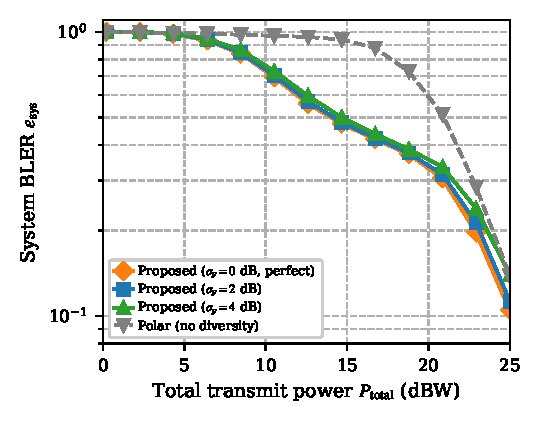
\includegraphics[width=0.7\columnwidth]{bler_robustness_prediction.eps}\\
{\small \textbf{Fig.~\ref{fig:bler_robustness}:} {\color{blue}System BLER versus total transmit power under imperfect
prediction with combined prediction error $\sigma_p$.}}
\end{center}

\begin{center}
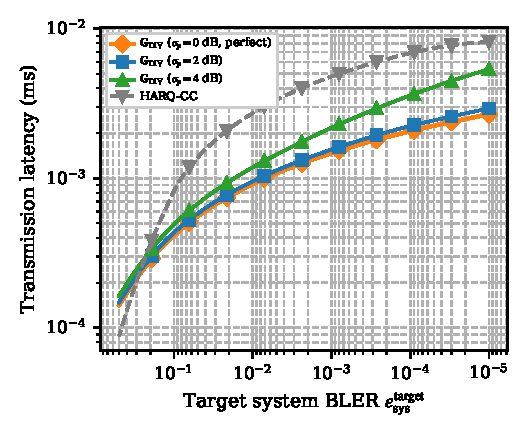
\includegraphics[width=0.7\columnwidth]{latency_robustness_prediction.eps}\\
{\small \textbf{Fig.~\ref{fig:latency_robustness}:} {\color{blue}Transmission latency versus target system BLER under
imperfect prediction at $P_{\mathrm{total}} = 10$~dBW.}}
\end{center}

The ephemeris prediction targets a future frame at time $t_{k+\Delta}$ (Eq.~\eqref{eq:predicted_path_loss}). Since the total system latency $T_\Delta$ is on the order of milliseconds while LEO orbital geometry changes over tens of seconds, the prediction horizon contributes negligible additional mismatch relative to the $\sigma_p$ values studied above. In summary, the BLER degrades by only ${\sim}3$ percentage points at $\sigma_p = 4$~dB, and the latency advantage over HARQ-CC is preserved across all evaluated $\sigma_p$ values.

We hope that the new robustness analysis and figures address this concern.


\subsection{Reviewer Comment-2}



\begin{mdframed}
\begin{quote}
Second, the manuscript repeatedly motivates the problem using simultaneous outages and correlated satellite visibility/blockage behavior, especially at low elevation. However, the high-SNR system BLER approximation in Corollary 2 is explicitly built on statistically independent subchannel failures, even though the algebraic recovery guarantee itself is correlation-agnostic. This creates a gap between the motivation and the system-level performance analysis. I strongly encourage the authors to add experiments with correlated outage models, for example common blockage states, correlated shadowing, or geometry-driven correlated low-elevation events, and to discuss how much of the reported gain survives under such conditions.

\end{quote}

\end{mdframed}


\subsection{Response}

We thank the reviewer for this important observation. We agree that the gap between the correlated-outage motivation and the independent-failure analysis needed to be addressed. In the revised manuscript, three changes have been made: (i) a Gaussian copula correlated blockage model has been added to Section~II-A that preserves the elevation-dependent marginal blockage probabilities while introducing pairwise spatial correlation $\rho_{\mathrm{blk}}$ across subchannels; (ii) we have clarified in Section~IV that the algebraic recovery guarantee of Theorem~2 holds irrespective of the correlation structure; and (iii) a new figure (Fig.~\ref{fig:bler_correlated_blockage}) evaluates the system BLER as $\rho_{\mathrm{blk}}$ increases from $0$ to $0.9$, showing that the diversity transform maintains the lowest BLER for moderate correlation ($\rho_{\mathrm{blk}} \leq 0.8$) and should be adaptively bypassed only under near-common blockage ($\rho_{\mathrm{blk}} > 0.85$). The following text and equation have been added to Section~II-A:

\begin{quote}
``{\color{blue}The preceding model treats blockage indicators
$\{B_{i,k\ell}(t)\}$ as independent across subchannels. In practice,
co-visible LEO satellites at similar low elevations share a common
obstruction environment, introducing spatial correlation in blockage
events. To capture this effect, we adopt a Gaussian copula model~\cite{Nelsen2006, Ghadi2021}. Let
$\mathbf{Z} = [Z_1, \ldots, Z_n]^\top \sim
\mathcal{N}(\mathbf{0}, \mathbf{R}_{\mathrm{blk}})$,
where the equicorrelation matrix has entries}
\begin{equation*}
\color{blue}
[\mathbf{R}_{\mathrm{blk}}]_{ij} = \begin{cases}
1, & i = j, \\
\rho_{\mathrm{blk}}, & i \neq j,
\end{cases}
\end{equation*}
{\color{blue}with $\rho_{\mathrm{blk}} \in [0,1]$. The blockage indicator of
subchannel~$i$ is then defined as
$B_i = \mathbf{1}\{\Phi(Z_i) \leq P_{\mathrm{LOS}}(\epsilon_i)\}$.
Each subchannel maintains its elevation-dependent marginal
blockage probability
$1 - P_{\mathrm{LOS}}(\epsilon_i)$ from~\eqref{eq:los_prob}, while
$\rho_{\mathrm{blk}}$ controls the degree of spatial correlation:
$\rho_{\mathrm{blk}} = 0$ recovers independent blockage, whereas
$\rho_{\mathrm{blk}} \to 1$ approaches a common-blockage scenario in
which all subchannels tend to be simultaneously obstructed.}''
\end{quote}

The following discussion and figure have been added to Section~V:

\begin{quote}
``{\color{blue}Fig.~\ref{fig:bler_correlated_blockage} evaluates the system
BLER as a function of the blockage correlation parameter
$\rho_{\mathrm{blk}}$ using the Gaussian copula model
in~\eqref{eq:corr_matrix_blk}, with a fixed per-subchannel blockage probability of $0.2$.
At $\rho_{\mathrm{blk}} = 0$, the diversity transform achieves substantially lower BLER than the baselines, consistent with the
independent-blockage results in Fig.~\ref{fig:bler_vs_blockage}.
As $\rho_{\mathrm{blk}}$ increases, the gap narrows because correlated blockage drives the failure
distribution toward two extremes: either all subchannels survive or all are simultaneously blocked. In the former case, the diversity transform
is unnecessary, whereas in the latter, no scheme can recover the data once
more than $f_{\max}$ subchannels are lost.
Consequently, the partial-failure regime, where the MDS recovery
guarantee of Theorem~\ref{thm:block_mds} is most effective, becomes less probable under strong correlation.
For moderate correlation
($\rho_{\mathrm{blk}} \leq 0.8$), the diversity transform
consistently achieves the lowest BLER.
Beyond $\rho_{\mathrm{blk}} \approx 0.85$, however, the baselines
outperform the diversity transform. In this regime, blockage events become nearly common across all subchannels, reducing the benefit of algebraic erasure protection. Consequently, the rate overhead of the MDS diversity
code ($\varrho/n_{\mathrm{out}} = 2/3$) outweighs its recovery gain.
This crossover indicates that the diversity transform is most
effective in the low-to-moderate correlation regime relevant to LEO NTN systems with spatially
separated satellites.  Accordingly, the diversity transform can be adaptively disabled when
the predicted correlation becomes very high $\ldots$}''
\end{quote}

\begin{center}
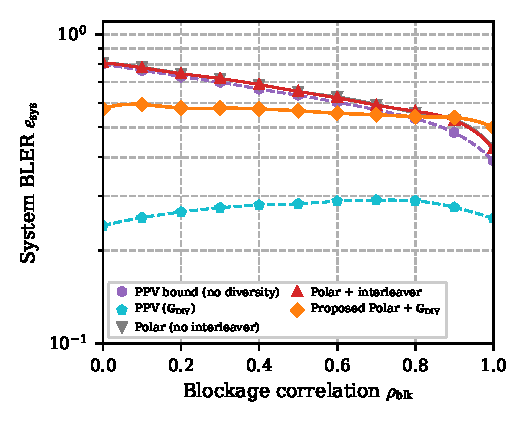
\includegraphics[width=0.7\columnwidth]{bler_vs_correlated_blockage.eps}\\
{\small \textbf{Fig.~\ref{fig:bler_correlated_blockage}:} {\color{blue}System BLER versus blockage correlation
$\rho_{\mathrm{blk}}$ at per-subchannel blockage probability $0.2$.}}
\end{center}

These results confirm that the reported gains survive under realistic correlated outage conditions ($\rho_{\mathrm{blk}} \leq 0.8$), and provide a clear design guideline: the diversity transform should be used when subchannels experience partially correlated blockage, and adaptively bypassed under near-common blockage.

We trust that the new correlated blockage model and simulation results satisfactorily address this point.


\subsection{Reviewer Comment-3}



\begin{mdframed}
\begin{quote}
Third, the OTFS part needs a more realistic impairment study. The manuscript explicitly notes that fractional Doppler and imperfect channel estimation may reduce the effective delay-Doppler diversity order, and later states that the analysis assumes integer Doppler indices. This limitation is too important to remain mostly a caveat in the text. Please quantify the performance gap under fractional Doppler and imperfect channel estimation, because this is directly tied to the claimed advantage over OFDM in high-mobility LEO settings.

\end{quote}

\end{mdframed}


\subsection{Response}

We thank the reviewer for raising this point. We agree that the impact of fractional Doppler and imperfect channel estimation needed to be quantified explicitly. In the revised manuscript, a new SINR impairment model has been added to Section~II-C that captures both fractional Doppler interference and channel estimation MSE through a single closed-form SINR expression. Two new curves have been added to Fig.~\ref{fig:otfs_vs_ofdm}, showing that fractional Doppler and imperfect CSI increase the BLER by approximately $1.5$--$2$ times relative to the ideal case, yet OTFS remains significantly below the OFDM curves at high normalised Doppler, confirming that the OTFS advantage and the diversity transform's recovery guarantee are both preserved under realistic impairments. To address this concern, a new analytical model has been added at the end of the OTFS Modulation subsection, Section~II-C:

\begin{quote}
``{\color{blue}The DD input--output relation in~\eqref{eq:dd_io} assumes
that each tap's Doppler shift aligns exactly with an integer DD bin.
When the physical Doppler $\nu_p$ of the $p$th tap does not coincide
with a grid point, a fractional offset
$\alpha_p = \nu_p - \lfloor\nu_p\rceil$ introduces inter-Doppler
interference with variance
$\sigma_{\mathrm{frac}}^2 = (\pi\,\alpha_p)^2/(3\,N_{\mathrm{D}})$~\cite{Raviteja2018,Moose1994}.
Under imperfect channel estimation with per-element MSE
$\sigma_{\mathrm{CSI}}^2$, the effective post-equalisation SINR is}
\begin{equation*}
\color{blue}
\gamma_i^{\mathrm{eff}} =
\frac{\gamma_i^{\mathrm{c}}}
{1 + \gamma_i^{\mathrm{c}}
\left(\sigma_{\mathrm{frac}}^2
+ \sigma_{\mathrm{CSI}}^2\right)}.
\end{equation*}
{\color{blue}Setting $\alpha_p = 0$ and $\sigma_{\mathrm{CSI}}^2 = 0$
recovers the ideal integer-Doppler, perfect-CSI case.}''
\end{quote}

The following discussion has been added to Section~V:

\begin{quote}
``$\ldots$ These results confirm that DD domain processing with OTFS, combined with the proposed diversity transform, is well suited to the high Doppler shifts characteristic of LEO satellite links.
{\color{blue}To quantify the impact of fractional Doppler and imperfect
channel estimation, Fig.~\ref{fig:otfs_vs_ofdm} also includes the
proposed OTFS scheme under two additional impairment conditions:
(i)~fractional Doppler with worst-case offset $\alpha_p = 0.5$ and perfect channel estimation; and
(ii)~fractional Doppler combined with imperfect channel estimation
($\sigma_{\mathrm{CSI}}^2 = 0.01$, corresponding to a channel estimation MSE of $-20$~dB, which is representative of embedded pilot-aided OTFS estimation at moderate SNR~\cite{Raviteja2018}).
Both impaired OTFS curves exhibit a moderate BLER increase (approximately
$1.5$--$2$ times) relative to the ideal integer-Doppler case, yet
remain significantly below the OFDM curves at high normalised Doppler.
This confirms that the OTFS advantage over OFDM is preserved under
realistic impairments, and that the diversity transform's
subchannel-level recovery guarantee of Theorem~\ref{thm:block_mds}
remains effective.}

\begin{center}
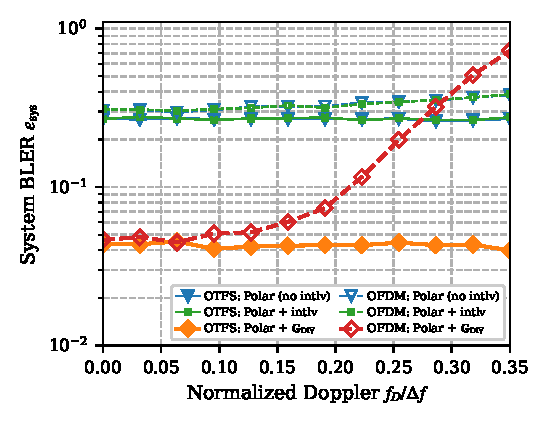
\includegraphics[width=0.7\columnwidth]{otfs_vs_ofdm.eps}\\
{\small \textbf{Fig.~\ref{fig:otfs_vs_ofdm}:} {\color{blue}BLER versus normalised Doppler $f_{D}/\Delta f$ for OTFS
and OFDM at $P_{\mathrm{total}} = 20$~dBW, including fractional
Doppler and imperfect channel estimation impairments.}}
\end{center}

In summary, the simulation results show that $\ldots$''
\end{quote}

These results directly quantify the performance gap requested by the reviewer: fractional Doppler and imperfect CSI increase the proposed scheme's BLER by approximately $1.5$ to $2$ times, while the OTFS advantage over OFDM and the diversity transform's recovery guarantee are both preserved.

We believe the new SINR impairment model and simulation curves quantify the impact of these practical impairments.


\subsection{Reviewer Comment-4}



\begin{mdframed}
\begin{quote}
Fourth, the system model relies heavily on the dominant feeder-link approximation. Table I and the numerical discussion state that the feeder-link SNR exceeds the access-link SNR by more than 39 dB, which justifies the simplifications used in the derivations. However, this also narrows the operating regime represented by the results. Please clarify more explicitly the applicability range of the theory when feeder-link degradation is non-negligible, especially under feeder-link weather impairment in Ka/Q-band operation. A sensitivity plot showing weaker feeder-link conditions would strengthen the paper considerably.

\end{quote}

\end{mdframed}


\subsection{Response}

We thank the reviewer for raising this important point. In the revised manuscript, three changes address this concern: (i) a footnote after Eq.~(16) in Section~II-B now states that the feeder-to-access SNR margin exceeds 39~dB under nominal conditions and remains above 27--34~dB under typical Ka-band rain attenuation of 5--12~dB, well above the 10~dB threshold at which the approximation begins to degrade; (ii) two simulation curves have been added to Fig.~\ref{fig:prop1_validation} for $n_c = 256$ under reduced feeder-link margins of 10~dB and 3~dB; and (iii) the results show that the BLER loss is less than 1.5~dB when the feeder-to-access margin exceeds 10~dB, with significant degradation appearing only below 10~dB---a regime typically mitigated through gateway diversity. The following footnote has been added after~\eqref{eq:combined_snr_final} in Section~II-B:

\begin{quote}
``{\color{blue}Under the parameters in Table~\ref{tab:sim_params}, the ratio $\bar{\gamma}_{i,\mathrm{GS}}/\bar{\gamma}_{i,\mathrm{SU}}$ exceeds 39~dB. According to ITU-R P.618~\cite{ITU-R_P618-14}, Ka-band rain attenuation at 99.9\% link availability for mid-latitude gateway sites is typically 5--12~dB, which reduces this margin to approximately 27--34~dB, well above the 10~dB threshold at which the approximation begins to degrade. The sensitivity of the subchannel BLER to reduced $\bar{\gamma}_{i,\mathrm{GS}}/\bar{\gamma}_{i,\mathrm{SU}}$ is quantified in Fig.~\ref{fig:prop1_validation}.}''
\end{quote}

The following discussion has been added to Section~V:

\begin{quote}
``{\color{blue}Fig.~\ref{fig:prop1_validation} also evaluates the sensitivity of the subchannel BLER to feeder-link degradation by showing simulation results for $n_c = 256$ with reduced feeder-to-access SNR margins of $\bar{\gamma}_{i,\mathrm{GS}}/\bar{\gamma}_{i,\mathrm{SU}} = 10$~dB and $3$~dB, corresponding to severe and extreme Ka-band rain fade conditions, respectively. The BLER loss is less than 1.5~dB when $\bar{\gamma}_{i,\mathrm{GS}}/\bar{\gamma}_{i,\mathrm{SU}}$ exceeds 10~dB, while significant degradation appears only when $\bar{\gamma}_{i,\mathrm{GS}}/\bar{\gamma}_{i,\mathrm{SU}}$ falls below 10~dB, a regime that corresponds to rain attenuation exceeding 30~dB and is typically mitigated through gateway diversity in operational systems.}''
\end{quote}

\begin{center}
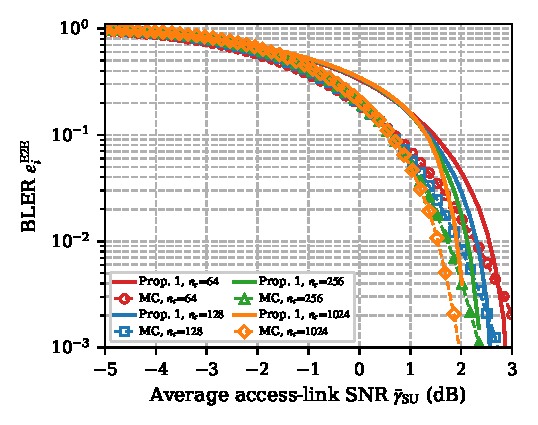
\includegraphics[width=0.7\columnwidth]{prop1_closedform_validation.eps}\\
{\small \textbf{Fig.~\ref{fig:prop1_validation}:} Subchannel BLER versus average access-link SNR for different per-subchannel blocklengths $n_c$ under dominant-LOS Rician fading: simulation and closed-form
  approximation in Proposition~\ref{prop:bler_approx}. {\color{blue}Feeder-link sensitivity is shown for $n_c = 256$ with $\bar{\gamma}_{i,\mathrm{GS}}/\bar{\gamma}_{i,\mathrm{SU}} = 10$~dB and $3$~dB.}}
\end{center}

These changes characterise the applicability range of the dominant feeder-link approximation and confirm that the theory remains accurate under realistic Ka-band weather impairment.

We hope that the added sensitivity curves and discussion clarify the applicability range of the feeder-link approximation.


\subsection{Reviewer Comment-5}



\begin{mdframed}
\begin{quote}
Fifth, the baseline section should be strengthened and made more explicit. The manuscript compares primarily against standalone polar coding, with and without interleaving, and later against OFDM under Doppler and HARQ-CC in terms of latency. This is useful, but the paper's main claim is about replacing conventional multi-connectivity diversity approaches that rely on statistical combining. Therefore, a more direct baseline discussion against satellite diversity with selection combining or MRC at the system level would improve fairness and sharpen the contribution. Even if a full new implementation is not added, the manuscript should explain more clearly why the current baselines are sufficient and what aspects are not being compared.

\end{quote}

\end{mdframed}


\subsection{Response}

We thank the reviewer for this suggestion. We agree that MRC and SC baselines are essential for a fair evaluation. In the revised manuscript, MRC and SC have been added to both the latency comparison (Fig.~\ref{fig:latency_comparison}) and the throughput comparison (Fig.~\ref{fig:throughput}). MRC combines LLRs from all non-blocked subchannels while SC selects the best subchannel; both repeat the same codeword on every subchannel and therefore require $k_c$ times more channel uses for the same message size. The diversity transform achieves the lowest latency among all four schemes (approximately three times lower than HARQ-CC at $P_{\mathrm{total}} = 10$~dBW and $\epsilon_{\mathrm{sys}}^{\mathrm{target}} = 10^{-3}$), and surpasses rate-optimised MRC in throughput at $P_{\mathrm{total}} \approx 12$~dBW, achieving nearly twice the MRC throughput at 25~dBW. The latency comparison discussion in Section~V now reads:

\begin{quote}
``Fig.~\ref{fig:latency_comparison} demonstrates the latency advantage of the diversity transform over {\color{blue}MRC, SC, and} the HARQ-CC baseline in~\eqref{eq:harq_bler}--\eqref{eq:harq_latency}{\color{blue}, configured with $K_{\max} = 4$, $T_{\mathrm{RTT}} = 20$~ms~\cite{3GPP38821}, and persistent blockage across retransmission attempts. Latency values are geometric means over channel realisations. MRC combines LLRs from all non-blocked subchannels (effective SNR $= \sum_j \bar{\gamma}_j$), and SC selects the subchannel with the highest instantaneous SNR; both repeat the same codeword on every subchannel and therefore require $k_c$ times more channel uses to deliver the same message size.} Despite the chase combining advantage, the diversity transform consistently achieves lower transmission latency than {\color{blue}all three baselines} across all operating points. {\color{blue}For example, at $P_{\mathrm{total}} = 10$~dBW and $\epsilon_{\mathrm{sys}}^{\mathrm{target}} = 10^{-3}$, the diversity transform achieves approximately three times lower latency than HARQ-CC.} As the target system BLER $\epsilon_{\mathrm{sys}}^{\mathrm{target}}$ becomes stricter, HARQ-CC latency grows faster because each additional retransmission round adds a full round-trip time{\color{blue}, while MRC and SC latency grows because their per-subchannel codeword must be $k_c$ times longer to deliver the same message}. This latency reduction follows directly from the single-shot decoding guarantee of Corollary~\ref{cor:latency_reduction} $\ldots$''
\end{quote}

\begin{center}
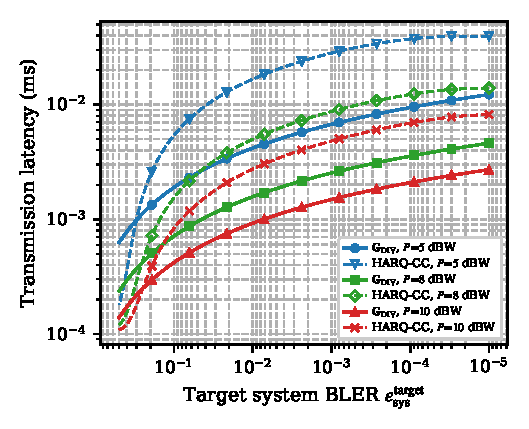
\includegraphics[width=0.7\columnwidth]{latency_comparison.eps}\\
{\small \textbf{Fig.~\ref{fig:latency_comparison}:} {\color{blue}Transmission latency versus target system BLER $\epsilon_{\mathrm{sys}}^{\mathrm{target}}$ for the diversity transform, MRC, SC, and HARQ-CC ($K_{\max} = 4$, $T_{\mathrm{RTT}} = 20$~ms) at $P_{\mathrm{total}} = 5$ and $10$~dBW. MRC and SC require $k_c = 4$ times more channel uses to deliver the same message size.}}
\end{center}

The throughput comparison in Section~V now reads:

\begin{center}
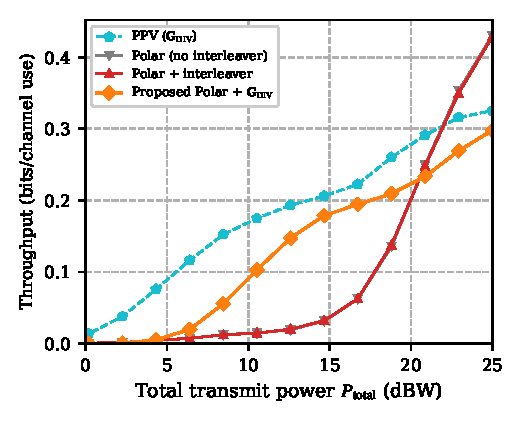
\includegraphics[width=0.7\columnwidth]{throughput_reliability.eps}\\
{\small \textbf{Fig.~\ref{fig:throughput}:} {\color{blue}Effective throughput versus total transmit power at $\epsilon = 40^{\circ}$ with $n_{\mathrm{s}} = 6$ subchannels. The diversity transform operates at effective rate $R_c \cdot \varrho/n_{\mathrm{out}} \approx 0.33$; per-subchannel baselines at $R_c = 0.5$. MRC and SC are rate-optimised at each power level.}}
\end{center}

We trust that the new MRC, SC, and HARQ-CC baselines in the throughput and latency figures strengthen the comparison.


\subsection{Reviewer Comment-6}



\begin{mdframed}
\begin{quote}
Sixth, the latency and throughput claims should be presented more carefully and transparently. The paper reports that the diversity-transform scheme can outperform the baselines in throughput over a medium-power regime despite operating at a lower effective code rate, and the conclusion claims more than 90\% reduction in median transmission latency for strict reliability targets. These are potentially strong results, but the presentation would be more convincing if the manuscript explicitly stated the exact HARQ-CC assumptions, maximum retransmission policy, latency metric definition, and representative numerical gains in the main text instead of leaving some of this implicit in the figure discussion.

\end{quote}

\end{mdframed}


\subsection{Response}

We thank the reviewer for this comment. We agree that the HARQ-CC assumptions and latency metric should be stated explicitly. In the revised manuscript, two changes have been made: (i) the HARQ-CC baseline has been formalised in Section~IV-D with explicit equations for the system BLER after $K_r+1$ attempts and the average transmission latency, including the chase combining SNR accumulation; and (ii) the discussion of Fig.~\ref{fig:latency_comparison} now explicitly states all configuration parameters ($K_{\max} = 4$, $T_{\mathrm{RTT}} = 20$~ms, persistent blockage, geometric mean latency) and representative numerical gains (approximately three times lower latency than HARQ-CC at $P_{\mathrm{total}} = 10$~dBW and $\epsilon_{\mathrm{sys}}^{\mathrm{target}} = 10^{-3}$). After Corollary~\ref{cor:latency_reduction}:

\begin{quote}
``$\ldots$ directly reducing the frame duration $T_{\mathrm{frame}}$ and
consequently the total system latency $T_{\Delta}$.

{\color{blue}For comparison, the conventional HARQ chase combining
(HARQ-CC) baseline operates as follows. After the $k$th
transmission attempt ($k = 0,\ldots,K_{\max}$), the receiver
combines all $k+1$ copies, yielding an effective SNR
$\gamma_{\mathrm{eff}} = \gamma \cdot (k+1)$.
The system BLER after $K_r+1$ attempts is}
\begin{equation*}
\color{blue}
\epsilon_{\mathrm{sys}}^{\mathrm{HARQ}} =
\prod_{k=0}^{K_r} \epsilon\!\left(\gamma(k{+}1),\, n_c,\, R_c\right),
\end{equation*}
{\color{blue}and the average transmission latency is}
\begin{equation*}
\color{blue}
\bar{T}_{\mathrm{HARQ}} = \sum_{k=0}^{K_r} p_k
\left(T_{\mathrm{frame}} + k\,T_{\mathrm{RTT}}\right),
\end{equation*}
{\color{blue}where $p_k$ is the probability of first successful decoding at
attempt~$k$ and $T_{\mathrm{RTT}}$ is the round-trip time.
The blocklength $n_c$ and retransmission count
$K_r \leq K_{\max}$ are jointly optimised to minimise
$\bar{T}_{\mathrm{HARQ}}$ subject to
$\epsilon_{\mathrm{sys}}^{\mathrm{HARQ}} \leq
\epsilon_{\mathrm{sys}}^{\mathrm{target}}$.}''
\end{quote}

The latency comparison in Section~V now reads:

\begin{quote}
``Fig.~\ref{fig:latency_comparison} demonstrates the latency advantage
of the diversity transform over {\color{blue}MRC, SC, and} the HARQ-CC baseline
in~\eqref{eq:harq_bler}--\eqref{eq:harq_latency}{\color{blue},
configured with $K_{\max} = 4$,
$T_{\mathrm{RTT}} = 20$~ms~\cite{3GPP38821}, and persistent
blockage across retransmission attempts.
Latency values are geometric means over channel realisations.
MRC combines LLRs from all non-blocked subchannels (effective SNR $= \sum_j \bar{\gamma}_j$), and SC selects the subchannel with the highest instantaneous SNR; both repeat the same codeword on every subchannel and therefore require $k_c$ times more channel uses to deliver the same message size.}
Despite the chase combining advantage, the diversity transform consistently achieves
lower transmission latency than {\color{blue}all three baselines} across all operating points.
{\color{blue}For example, at $P_{\mathrm{total}} = 10$~dBW and $\epsilon_{\mathrm{sys}}^{\mathrm{target}} = 10^{-3}$, the diversity transform achieves approximately three times lower latency than HARQ-CC.} $\ldots$''
\end{quote}

We hope that the explicit HARQ-CC model and numerical gain now provide the transparency requested.


\subsection{Reviewer Comment-7}



\begin{mdframed}
\begin{quote}
Seventh, a transactions paper should also comment on implementation cost. The manuscript highlights "single-pass diversity demapping and FEC decoding," but it does not provide much discussion of encoder/decoder complexity, transform construction/update overhead, memory footprint, or signaling overhead when the transform changes with the predicted outage family. A short complexity discussion, even if asymptotic, would improve the practical value of the paper.

\end{quote}

\end{mdframed}


\subsection{Response}

We thank the reviewer for this suggestion. A new subsection, Section~IV-F, ``Implementation Complexity,'' has been added to the revised manuscript, covering four aspects: (i) encoding/decoding complexity---the diversity layer adds $O(\varrho \cdot n_{\mathrm{out}} \cdot n_c)$ binary operations, negligible compared to the $O(\varrho \cdot L \cdot N \log N)$ SCL decoding cost; (ii) transform construction---executed once offline, with only a table index selection required per frame; (iii) memory footprint---polynomial in the MDS parameters and negligible relative to SCL path storage; and (iv) signalling overhead---at most $\lceil\log_2\binom{n_{\mathrm{s}}}{k_{\mathrm{c}}}\rceil$ bits per frame, or zero if both ends compute the erasure family independently from shared ephemeris data. In Section~IV-F, immediately before Section~\ref{sec:results}:

\begin{quote}
``$\ldots$ yielding a corresponding increase in the frame duration
$\check{T}_{\mathrm{frame}}(\sigma_p) =
\check{n}_c^{*}(\sigma_p)/(M_{\mathrm{D}}\Delta f)$.

{\color{blue}\textbf{Encoding and Decoding Complexity.}
At the transmitter, the diversity mapper computes
$\mathbf{Z} = G_{\mathrm{DIV}}^{\mathsf{T}}\,\mathbf{X}$, where
$\mathbf{X} \in \mathbb{F}_2^{\varrho \times n_c}$ contains the
$\varrho$ polar-encoded subwords. Since $G_{\mathrm{DIV}}$ is binary,
each entry of $\mathbf{Z}$ is obtained by XOR-ing at most $\varrho$
bits, yielding a total of
$O(\varrho \cdot n_{\mathrm{out}} \cdot n_c)$ binary additions.
At the receiver, diversity demapping applies a precomputed binary
recovery matrix
$G_{\mathrm{DIV}}^{\dagger}(E^c) \in
\mathbb{F}_2^{\varrho \times |E^c|}$
at the same asymptotic cost. For $n_c = N$, the diversity layer cost
$O(\varrho\, n_{\mathrm{out}}\, N)$ is typically much smaller than
the total SCL decoding cost $O(\varrho\, L\, N \log N)$, since
$L \log N \gg n_{\mathrm{out}}$ in practical settings. Consequently, the diversity demapping adds negligible
processing latency to the decoding pipeline, preserving the
single-pass receiver architecture described in
Section~\ref{subsec:receiver_demapping}.}

{\color{blue}\textbf{Transform Construction and Update Overhead.}
The RS--Vandermonde construction in
Algorithm~\ref{alg:div_transform_construction} requires
$O(k_{\mathrm{c}} \cdot n_{\mathrm{s}} \cdot m^2)$ finite-field
multiplications to build $G_{\mathrm{MDS}}$ and compute the faithful
binary representation. This computation is executed once offline,
together with all $\binom{n_{\mathrm{s}}}{k_{\mathrm{c}}}$ recovery
matrices, one per admissible erasure pattern, which are stored in a
lookup table.
Since the MDS code parameters $(k_{\mathrm{c}}, n_{\mathrm{s}}, m)$
are fixed for a given system configuration, the matrix
$G_{\mathrm{DIV}}$ itself remains static across frames.
At each frame, the ephemeris-driven predictor in
Section~\ref{sec:ephemeris_prediction} computes per-subchannel
BLER estimates $\tilde{\epsilon}_{i}^{\mathrm{E2E}}$ and
identifies which subchannels exceed the erasure threshold
$\epsilon_{\mathrm{th}}$, producing the predicted outage set
$S_{\mathrm{out}}$ in~\eqref{eq:outage_set}. The receiver then
selects the corresponding precomputed recovery matrix from the
lookup table indexed by $S_{\mathrm{out}}$. Thus, the only
per-frame update is a table index selection, not a matrix
recomputation.}

{\color{blue}\textbf{Memory Footprint.}
The binary diversity transform matrix
$G_{\mathrm{DIV}} \in \mathbb{F}_2^{\varrho \times n_{\mathrm{out}}}$
requires $\varrho \cdot n_{\mathrm{out}}$ bits of storage.
The precomputed recovery matrices, one for each of the
$\binom{n_{\mathrm{s}}}{k_{\mathrm{c}}}$ erasure patterns and
each of size $\varrho \times \varrho$ bits, add
$\binom{n_{\mathrm{s}}}{k_{\mathrm{c}}} \cdot \varrho^2$ bits.
Both quantities scale polynomially in the MDS code parameters and
are negligible compared to the $O(L \cdot N)$ bits required for
SCL decoding path storage.}

{\color{blue}\textbf{Signalling Overhead.}
The diversity transform is determined by the MDS code parameters
$(k_{\mathrm{c}}, n_{\mathrm{s}}, m)$ and the predicted erasure
family $\mathcal{E}_{\mathrm{robust}}$. Since both the gateway
and the UE share ephemeris data
(Section~\ref{sec:ephemeris_prediction}), the erasure family can
be independently computed at both ends without explicit signalling.
In operational scenarios where signalling is preferred for
robustness, the active erasure pattern index requires at most
$\lceil\log_2\binom{n_{\mathrm{s}}}{k_{\mathrm{c}}}\rceil$ bits
per OTFS frame, which is negligible relative to the $n_c$ coded
symbols transmitted per subchannel.}''
\end{quote}

We believe the new complexity subsection provides the practical assessment requested.


\subsection{Reviewer Comment-8}



\begin{mdframed}
\begin{quote}
On presentation, the paper is generally readable, but it is dense. The notation is heavy and sometimes the distinction between variables such as $n$, $ns$, $N_{serv}$, kc, $\rho$, and $nout$ is harder to follow than necessary. I suggest adding a compact notation table and tightening some of the longer explanatory paragraphs in Sections II–IV. The English is understandable, but it would benefit from another round of polishing for conciseness and grammar. Figure captions could also be slightly more self-contained.
In summary, I think the paper has real merit: the core algebraic idea is interesting, the finite-blocklength angle is valuable, and the problem is relevant. However, the current version still falls short of the level of practical validation and scope clarification I would expect for acceptance. I therefore recommend a major revision. If the authors can add robustness experiments for imperfect prediction and correlated outages, quantify the impact of fractional Doppler/channel-estimation errors, and clarify the scope, baselines, and implementation cost, the paper could become much stronger.
\end{quote}

\end{mdframed}


\subsection{Response}

We thank the reviewer for the presentation suggestions and for the constructive summary. All three presentation improvements have been implemented in the revised manuscript: (i) a compact notation table (Table~\ref{tab:notation}) has been added at the end of Section~I, listing all key system-level symbols; (ii) the dense paragraphs in Sections~II--IV have been tightened for conciseness; and (iii) figure captions now include key operating parameters for self-containedness. The manuscript has also undergone a complete round of English proofreading and grammar correction. Regarding the broader concerns summarised by the reviewer---practical validation, scope clarification, baselines, and implementation cost---we believe these are now comprehensively addressed through the new robustness analysis (Comment~1), correlated blockage model (Comment~2), fractional Doppler and CSI impairment quantification (Comment~3), feeder-link sensitivity study (Comment~4), expanded MRC/SC/HARQ-CC baselines (Comment~5), formalised HARQ-CC model with explicit parameters (Comment~6), and implementation complexity subsection (Comment~7). Details of each presentation change are provided below.

\textbf{1) Compact notation table.}
Table~\ref{tab:notation} has been added at the end of Section~I, summarising all key system-level symbols so that the reader can quickly cross-reference symbol meanings.

\begin{center}
{\color{blue}
\begin{tabular}{@{}cl@{}}
\toprule
\textbf{Symbol} & \textbf{Description} \\
\midrule
$n$ ($= N_{\text{serv}}$) & Number of physical subchannels (serving satellites) \\
$n_{\mathrm{s}}$ & RS code length (number of field-symbol blocks) \\
$k_{\mathrm{c}}$ & RS code dimension (minimum surviving blocks) \\
$m$ & Extension degree of $\mathbb{F}_{2^m}$ \\
$d_{\min}$ & MDS minimum distance ($= n_{\mathrm{s}} - k_{\mathrm{c}} + 1$) \\
$\varrho$ & Number of encoder subwords ($= k_{\mathrm{c}} m$) \\
$n_{\text{out}}$ & Number of diversity transform outputs ($= n_{\mathrm{s}} m$) \\
$G_{\mathrm{DIV}}$ & Binary diversity transform matrix ($\varrho \times n_{\text{out}}$) \\
$N_{\mathrm{D}}, M_{\mathrm{D}}$ & OTFS Doppler and delay grid dimensions \\
$n_c$ & OTFS frame blocklength ($= N_{\mathrm{D}} M_{\mathrm{D}}$) \\
$(N, K)$ & Polar code length and information bits \\
$R_c$ & Polar code rate ($= K/N$) \\
$L$ & SCL decoder list size \\
$\epsilon_i^{\mathrm{E2E}}$ & Per-subchannel end-to-end BLER \\
$\epsilon_{\mathrm{sys}}$ & Overall system BLER \\
$f_{\max}$ & Maximum tolerable subchannel failures ($= n - k_{\mathrm{c}}$) \\
$\gamma_i^{\mathrm{c}}$ & Combined end-to-end SNR of subchannel $i$ \\
$P_{\mathrm{total}}$ & Total transmit power \\
$T_{\Delta}$ & Total system latency \\
$\epsilon_{\mathrm{th}}$ & Erasure declaration threshold \\
$\sigma_p$ & Prediction error standard deviation (dB) \\
$\rho_{\mathrm{blk}}$ & Blockage correlation parameter \\
\bottomrule
\end{tabular}
}
\end{center}

\textbf{2) Tightened paragraphs in Sections~II--IV.}
We have revised the dense paragraphs identified by the reviewer.

The finite-blocklength BLER introduction (Section~III-A) now reads:

\begin{quote}
``{\color{blue}The per-subchannel BLER is derived using finite blocklength information theory, accounting for the cascaded relay structure, OTFS-enabled multipath diversity, and the blocklength penalty. A subchannel is in outage when its end-to-end error probability exceeds the target threshold $\epsilon_{\mathrm{th}}$. For an OTFS frame with blocklength $n_c = N_{\mathrm{D}} M_{\mathrm{D}}$, the DD-domain structure provides diversity across the $L_i$ resolvable access-link paths $\ldots$}''
\end{quote}

The diversity transform recovery guarantee (Section~IV) now reads:

\begin{quote}
``{\color{blue}To ensure robustness against subchannel outages, the diversity transform matrix $G_{\mathrm{DIV}} \in \mathbb{F}_2^{\varrho \times n_{\text{out}}}$ is designed such that $\mathrm{rank}\!\left(G_{\mathrm{DIV}}(E^{c})\right)=\varrho$ for all erasure patterns $E$
satisfying $|\{i : A_i \subseteq E\}| \leq f_{\mathrm{max}}^{\mathrm{sys}}$. This condition guarantees
complete recovery of $\varrho$ information subwords under any combination of $f_{\mathrm{max}}^{\mathrm{sys}}$ subchannel failures, regardless of whether the outages were predicted. Since the predicted erasure family $\mathcal{E}_{\mathrm{robust}}[k+\Delta]$ in~\eqref{eq:erasure_pattern} is a subset of these guaranteed recoverable patterns, the proposed transform also provides robustness against unexpected outages. The algebraic construction based on MDS codes is presented in Section~\ref{sec:diversity_transform_construction}.}''
\end{quote}

\textbf{3) Self-contained figure captions.}
The captions of Figs.~\ref{fig:bler_vs_elevation}, \ref{fig:bler_vs_blockage}, \ref{fig:throughput}, and~\ref{fig:latency_comparison} now include the key operating parameters:

\begin{quote}
``{\color{blue}Fig.~\ref{fig:bler_vs_elevation}: System BLER versus elevation angle $\epsilon$ at $P_{\mathrm{total}} = 8$~dBW with $n_{\mathrm{s}} = 6$ subchannels and $(N,K) = (256,128)$ polar code.}''
\end{quote}

\begin{quote}
``{\color{blue}Fig.~\ref{fig:bler_vs_blockage}: System BLER versus per-subchannel blockage probability at $P_{\mathrm{total}} = 8$~dBW with $n_{\mathrm{s}} = 6$ subchannels and $d_{\min} = 3$.}''
\end{quote}

\begin{quote}
``{\color{blue}Fig.~\ref{fig:throughput}: Effective throughput versus total transmit power at $\epsilon = 40^{\circ}$ with $n_{\mathrm{s}} = 6$ subchannels. The diversity transform operates at effective rate $R_c \cdot \varrho/n_{\mathrm{out}} \approx 0.33$; per-subchannel baselines at $R_c = 0.5$. MRC and SC are rate-optimised at each power level.}''
\end{quote}

\begin{quote}
``{\color{blue}Fig.~\ref{fig:latency_comparison}: Transmission latency versus target system BLER $\epsilon_{\mathrm{sys}}^{\mathrm{target}}$ for the diversity transform, MRC, SC, and HARQ-CC ($K_{\max} = 4$, $T_{\mathrm{RTT}} = 20$~ms) at $P_{\mathrm{total}} = 5$ and $10$~dBW. MRC and SC require $k_c = 4$ times more channel uses to deliver the same message size.}''
\end{quote}

We hope that these presentation improvements, together with the substantive technical revisions described in Comments~1--7, address all concerns raised.

\vskip 0.2in
We sincerely appreciate the time and effort you have dedicated to reviewing our manuscript. Your detailed comments have been instrumental in strengthening the paper. We remain committed to making any further adjustments as needed.
%%%%%%%%%%%%%%%%%%%%%%%%%%%%%%%%%%%%%%%%%%%%%%%%%%%%%%%%%%%%%%%%%%%%%%
